\caulc
\begin{ex}%[1D3N2-5]%[TDMZZ28]%[Võ Hiệp]
	Giới hạn $\lim\limits_{x \to +\infty} \left( \dfrac{4x^2 + 3}{x^2 - 1} \right)$ bằng
	\choice
	{$-3$}
	{$0$}
	{\True $4$}
	{$+\infty$}
	\loigiai{
		Ta có
		$\lim\limits_{x \to +\infty} \dfrac{4x^2 + 3}{x^2 - 1} = \lim\limits_{x \to +\infty} \dfrac{4 + \dfrac{3}{x^2}}{1 - \dfrac{1}{x^2}} = 4$.
	}
\end{ex}

\begin{ex}%[1H8N7-1]%[TDMZZ28]%[Võ Hiệp]
	Thể tích của khối chóp có diện tích đáy bằng $6$ và chiều cao bằng $2$ là
	\choice
	{\True $V = 4$}
	{$V = 12$}
	{$6$}
	{$V = 24$}
	\loigiai{
		Thể tích của khối chóp là
		$V = \dfrac{1}{3} B \cdot h = \dfrac{1}{3} \cdot 6 \cdot 2 = 4$.
	}
\end{ex}

\begin{ex}%[1D6H4-2]%[TDMZZ28]%[Võ Hiệp]
	Tập nghiệm của phương trình $\log_2\left(x^2 - 1\right) = 3$ là
	\choice
	{$\{3\}$}
	{\True $\{\pm 3\}$}
	{$\{-3\}$}
	{$\left\{\pm \sqrt{7}\right\}$}
	\loigiai{
		Điều kiện xác định $x^2 - 1 > 0 \Leftrightarrow x^2 > 1$.\\
		Phương trình đã cho tương đương với
		$x^2 - 1 = 2^3 \Leftrightarrow x^2 - 1 = 8 \Leftrightarrow x^2 = 9 \Leftrightarrow x = \pm 3$ (thỏa mãn).\\
		Vậy tập nghiệm của phương trình là $S = \{\pm 3\}$.
	}
\end{ex}

\begin{ex}%[1D7H2-1]%[TDMZZ28]%[Võ Hiệp]
	Đạo hàm của hàm số $y = \mathrm{e}^{3x}$ là
	\choice
	{$y' = \mathrm{e}^{3x}$}
	{\True $y' = 3\mathrm{e}^{3x}$}
	{$y' = \dfrac{\mathrm{e}^{3x}}{3}$}
	{$y' = \mathrm{e}^{9x}$}
	\loigiai{
		Ta có
		$y' = \left(\mathrm{e}^{3x}\right)' = (3x)' \cdot \mathrm{e}^{3x} = 3\mathrm{e}^{3x}$.
	}
\end{ex}

\begin{ex}%[2D1N4-1]%[TDMZZ28]%[Võ Hiệp]
	Đường tiệm cận đứng của đồ thị hàm số $y = \dfrac{1}{2x - 3}$ là
	\choice
	{$x = 3$}
	{$y = \dfrac{1}{2}$}
	{$y = \dfrac{3}{2}$}
	{\True $x = \dfrac{3}{2}$}
	\loigiai{
		Ta có $\lim\limits_{x\to\left(\tfrac{3}{2}\right)^-}\dfrac{1}{2x - 3}=-\infty$ và 	$\lim\limits_{x\to\left(\tfrac{3}{2}\right)^+}\dfrac{1}{2x - 3}=+\infty$.\\
		Do đó tiệm cận đứng của đồ thị hàm số $y = \dfrac{1}{2x - 3}$ là $x=\dfrac{3}{2}$.
		
	}
\end{ex}

\begin{ex}%[2D1H2-1]%[TDMZZ28]%[Võ Hiệp]
	Cho hàm số $y = f(x)$ có biểu thức đạo hàm $f'(x) = (x - 1)(x^2 - 4x + 3)$, $\forall x \in \mathbb{R}$. Số điểm cực trị của hàm số $f(x)$ là
	\choice
	{$3$}
	{$2$}
	{\True $1$}
	{$0$}
	\loigiai{
		Ta có $f'(x)=0\Leftrightarrow (x - 1)(x^2 - 4x + 3)=0\Leftrightarrow \hoac{&x-1=0\\&x^2 - 4x + 3}\Leftrightarrow \hoac{&x=1\\&\hoac{&x=1\\&x=3}}\Leftrightarrow \hoac{&x=1\\&x=3.}$\\
		Bảng xét dấu
		\begin{center}
			
\begin{tikzpicture}[>=stealth,line join=round,line cap=round,font=\footnotesize,scale=1]
				\tkzTabInit[nocadre=true,lgt=1.2,espcl=2.2,deltacl=0.6]
				{$x$/1,$f'(x)$/1}
				{$-\infty$,$1$,$3$,$+\infty$}
				\tkzTabLine{,-,0,-,0,+,}
			\end{tikzpicture}
		\end{center}
		Suy ra hàm số $f(x)$ chỉ có đúng $1$ điểm cực trị tại $x = 3$.
	}
\end{ex}

\begin{ex}%[2H2H1-3]%[TDMZZ28]%[Võ Hiệp]
	\immini[thm]{
		Cho hình lập phương $ABCD. A'B'C'D'$. Đáp án nhận xét \textbf{sai} là
		\choice
		{$\overrightarrow{AB}\cdot \overrightarrow{CC'}=0$}
		{$\overrightarrow{AC}\cdot \overrightarrow{BD'}=0$}
		{\True $\overrightarrow{AB'}\cdot \overrightarrow{A'D}=0$}
		{$\overrightarrow{AB}\cdot \overrightarrow{B'C}=0$}
	}{
		\begin{tikzpicture}[scale=.7,>=stealth, font=\footnotesize, line join=round, line cap=round]
			\def\a{3.5}
			\path 	(0:0) coordinate (A)
			++(0:\a) coordinate (D)
			++(-130:\a/2) coordinate (C)
			($(A)+(C)-(D)$) coordinate (B)
			($(A)+(90:\a)$) coordinate (A')
			($(B)+(90:\a)$) coordinate (B')
			($(C)+(90:\a)$) coordinate (C')
			($(D)+(90:\a)$) coordinate (D');
			\draw[dashed] 	(B)--(A)--(D)	(A)--(A');
			\draw 	(C)--(C') 	(D)--(D') 	(B)--(B') 	(B)--(C)--(D) (A')--(B')--(C')--(D')--cycle;
			\foreach \x/\g in {A/180,B/180,C/0,D/0,A'/180,B'/180,C'/0,D'/0}
			\fill[black] 	(\x) circle (1pt)
			($(\g:4mm)+(\x)$) node {$\x$};	
		\end{tikzpicture}
	}
	\loigiai{
		Vì $ABCD. A'B'C'D'$ là hình lập phương nên ta có
		\begin{itemize}
			\item $AB\perp (BB'C'C)\Rightarrow AB\perp CC'\Rightarrow\overrightarrow{AB}\perp \overrightarrow{CC'}\Rightarrow\overrightarrow{AB}\cdot \overrightarrow{CC'}=0$.
			\item $AC\perp (BB'D'D)\Rightarrow AC\perp BD'\Rightarrow \overrightarrow{AC}\perp \overrightarrow{BD'}\Rightarrow\overrightarrow{AC}\cdot \overrightarrow{BD'}=0$.
			\item $\heva{&(AB',B'C)=60^\circ\\&B'C\parallel A'D}\Rightarrow (AB',A'D)=60^\circ \Rightarrow\overrightarrow{AB'}\cdot \overrightarrow{B'D}\ne 0$.
			\item $AB\perp (BB'C'C)\Rightarrow AB\perp B'C\Rightarrow\overrightarrow{AB}\perp \overrightarrow{B'C}\Rightarrow\overrightarrow{AB}\cdot \overrightarrow{B'C}=0$.
		\end{itemize}
		
	}
\end{ex}

\begin{ex}%[2D4N1-3]%[TDMZZ28]%[Võ Hiệp]
	Họ nguyên hàm của hàm số $f(x)=\sin x$ là
	\choice
	{\True $F(x)=-\cos x + C$}
	{$F(x)=\cos x + C$}
	{$F(x)=\tan x + C$}
	{$F(x)=\dfrac{1}{2}\sin^2 x + C$}
	\loigiai{
		Ta có $\displaystyle\int\limits \sin x \mathrm{\,d}x=-\cos x + C$.
	}
\end{ex}

\begin{ex}%[2H5N3-2]%[TDMZZ28]%[Võ Hiệp]
	Trong không gian $Oxyz$, cho mặt cầu $(S)\colon x^2 + y^2 + z^2 + 2x + 2y = 0$. Tọa độ tâm của mặt cầu $(S)$ là
	\choice
	{\True $(-1;-1;0)$}
	{$(1;1;0)$}
	{$(0;1;0)$}
	{$(2;2;-2023)$}
	\loigiai{
		Từ phương trình mặt cầu $(S)\colon x^2 + y^2 + z^2 + 2x + 2y = 0$, ta có
		$\heva{& -2a = 2 \\ &-2b = 2 \\ &-2c = 0}\Leftrightarrow \heva{&a = -1 \\ &b = -1 \\ &c = 0. }$\\
		Vậy tọa độ tâm của mặt cầu $(S)$ là $I(-1;-1;0)$.
	}
\end{ex}

\begin{ex}%[0D0H2-2]%[TDMZZ28]%[Võ Hiệp]
	Gieo một con súc sắc cân đối đồng chất $2$ lần liên tiếp. Tính xác suất để tổng số chấm xuất hiện trong $2$ lần gieo là một số tự nhiên chia hết cho $5$.
	\choice
	{$\dfrac{1}{9}$}
	{$\dfrac{2}{9}$}
	{$\dfrac{2}{13}$}
	{\True $\dfrac{7}{36}$}
	\loigiai{
		Số phần tử của không gian mẫu khi gieo con súc sắc $2$ lần liên tiếp là $n(\Omega) = 6 \cdot 6 = 36$.\\
		Gọi $A$ là biến cố \lq\lq Tổng số chấm xuất hiện trong $2$ lần gieo là một số tự nhiên chia hết cho $5$\rq\rq.\\
		Ta có $A=\{(1; 4), (2; 3), (3; 2), (4; 1), (4; 6), (5; 5), (6; 4) \}$.\\
		Số kết quả thuận lợi cho biến cố $A$ là $n(A) = 7$.\\
		Xác suất của biến cố $A$ là $\mathrm{P}(A)= \dfrac{n(A)}{n(\Omega)} = \dfrac{7}{36}$.
	}
\end{ex}

\begin{ex}%[2D1H2-1]%[TDMZZ28]%[Võ Hiệp]
	Số điểm cực trị của đạo hàm của hàm số $f(x)=x^4-4x^2+3$ là
	\choice
	{$3$}
	{\True $2$}
	{$1$}
	{$0$}
	\loigiai{
		Tập xác định $\mathscr{D}=\mathbb{R}$.
		Ta có $f'(x) = 4x^3 - 8x$. \\
		Xét hàm số $g(x)=4x^3 - 8x$ trên $\mathbb{R}$.\\
		Ta có $g'(x)=12x^2-8$. Cho $g'(x)=0\Leftrightarrow 12x^2-8\Leftrightarrow \hoac{&x=-\dfrac{\sqrt{6}}{3}\\&x=\dfrac{\sqrt{6}}{3}.}$\\
		Bảng biến thiên hàm số $g(x)$
		\begin{center}
			
\begin{tikzpicture}[scale=1, line join=round, line cap=round, >=stealth, font=\footnotesize]	 
				\tkzTabInit[nocadre=true,lgt=1,espcl=2.5,deltacl=0.6]
				{$x$/.7, $g'(x) $/.7, $g(x) $/2.2}	
				{$-\infty$,$-\tfrac{\sqrt{6}}{3}$,$\tfrac{\sqrt{6}}{3}$,$+\infty$}
				\tkzTabLine{,+,0,-,0,+,} %h là tô nền
				\tkzTabVar{-/$-\infty$, +/$\dfrac{16\sqrt{6}}{9}$,-/$-\dfrac{16\sqrt{6}}{9}$,+/$+\infty$}
			\end{tikzpicture}
		\end{center}
		Vậy đạo hàm của hàm số $f(x)$ có $2$ điểm cực trị.
	}
\end{ex}

\begin{ex}%[2H5H2-6]%[TDMZZ28]%[Võ Hiệp]
	Trong không gian $Oxyz$, cho đường thẳng $d\colon \dfrac{x-1}{3}=\dfrac{y-2}{-1}=\dfrac{z+2}{2}$ và điểm $A(-1;2;0)$. Hình chiếu vuông góc của $A$ lên đường thẳng $d$ có hoành độ là
	\choice
	{$\dfrac{15}{7}$}
	{\True $\dfrac{4}{7}$}
	{$-\dfrac{16}{7}$}
	{$-\dfrac{1}{7}$}
	\loigiai{
		Phương trình tham số của đường thẳng $d$ là
		$\heva{&x = 1 + 3t \\ &y = 2 - t \\ &z = -2 + 2t.}$\\
		Gọi $H$ là hình chiếu vuông góc của $A$ lên đường thẳng $d$.\\
		Vì $H \in d$ nên $H(1+3t; 2-t; -2+2t)\Rightarrow\overrightarrow{AH} = (2+3t; -t; -2+2t)$.\\
		Vectơ chỉ phương của đường thẳng $d$ là $\overrightarrow{u}_d = (3; -1; 2)$.\\
		Ta có
		\allowdisplaybreaks
		\begin{eqnarray*}
			AH \perp d
			&\Leftrightarrow& \overrightarrow{AH} \cdot \overrightarrow{u}_d = 0\\
			&\Leftrightarrow& 3(2+3t) - 1(-t) + 2(-2+2t) = 0\\
			&\Leftrightarrow& 14t + 2 = 0\\
			&\Leftrightarrow& t = -\dfrac{1}{7}.
		\end{eqnarray*}
		Hoành độ của điểm $H$ là $x_H = 1 + 3t = 1 + 3 \cdot \left(-\dfrac{1}{7}\right) = \dfrac{4}{7}$.
	}
\end{ex}
\cauds
\begin{ex}%[2D1H3-2]%[Dương Công Tạo]
	Trong mặt phẳng toạ độ $Oxy$, cho hàm số $y = x - 2026\ln x$ có đồ thị $(C)$.
	\choiceTF
	{\True Tập xác định của hàm số là $\mathscr{D} = (0;+\infty)$}
	{$f'(x)=1-2\,026x$}
	{$(C)$ có đúng một điểm cực đại}
	{$\min f (x) = -13\,400$}
	\loigiai{
		\begin{itemchoice}
			\itemch Tập xác định của hàm số là $\mathscr{D} = (0;+\infty)$.
			\itemch Với $x>0$, ta có $f'(x)=1-\dfrac{2\,026}{x}=\dfrac{x-2\,026}{x}$.
			\itemch $f'(x)=0\Leftrightarrow x-2\,026=0\Leftrightarrow x=2\,026$.\\
			Bảng biến thiên
			\begin{center}
				
\begin{tikzpicture}[>=stealth]
					\tkzTabInit[nocadre=false,lgt=1.5,espcl=2,deltacl=0.6]{$x$/.7 ,$f'(x)$/.7,$f(x)$/2}
					{$0$ , $2\,026$ , $+\infty$}
					\tkzTabLine{- , $0$ , + , }
					\tkzTabVar{+/$+\infty$ , -/$y_{\text{CT}}$ , +/$+\infty$}
				\end{tikzpicture}
			\end{center}
			Dựa vào bảng biến thiên, ta thấy hàm số đã cho đạt cực tiểu tại $x=2\,026$.
			\itemch Dựa vào bảng biến thiên, ta có $\lim\limits_{(0;+\infty)}y=f(2\,026)=2\,026-2\,026\ln2\,026\approx -13\,399{,}6$.
		\end{itemchoice}
	}
\end{ex}

\begin{ex}%[TDMZZ28]%[Hà Văn Hảo]%[2D6V2-4]
	Trong một buổi hội thảo chuyên đề về ứng dụng Trí tuệ nhân tạo AI trong học tập, có $200$ học sinh khối $11$ và $300$ học sinh khối $12$ tham gia. Qua khảo sát thực tế, tỉ lệ học sinh khối $11$ có sử dụng hệ thống AI hỗ trợ học tập là $0{,}3$; trong khi tỉ lệ này ở khối $12$ là $0{,}6$. Ban tổ chức chọn ngẫu nhiên một học sinh tham dự hội thảo để phỏng vấn.
	\choiceTF
	{\True Xác suất để học sinh được chọn tham gia phỏng vấn thuộc khối $12$ là $0{,}6$}
	{Xác suất để chọn được một học sinh của khối $12$ và em này có sử dụng AI là $0{,}18$}
	{Xác suất để học sinh được chọn có sử dụng AI là $0{,}66$}
	{Giả sử học sinh được chọn phỏng vấn cho biết mình có sử dụng AI, xác suất học sinh đó thuộc khối $12$ là $0{,}8$}
	\loigiai{
		Tổng số học sinh tham gia hội thảo là $200 + 300 = 500$ học sinh.\\
		Gọi các biến cố:\\
		- $A$: \lq\lq Học sinh được chọn thuộc khối $11$\rq\rq.\\
		- $B$: \lq\lq Học sinh được chọn thuộc khối $12$\rq\rq.\\
		- $X$: \lq\lq Học sinh được chọn có sử dụng AI\rq\rq.\\
		Ta xác định các xác suất ban đầu\\
		- Xác suất chọn được học sinh khối 11 là $\mathrm{P}(A) = \dfrac{200}{500} = 0{,}4$.\\
		- Xác suất chọn được học sinh khối 12 là $\mathrm{P}(B) = \dfrac{300}{500} = 0{,}6$.\\
		- Xác suất học sinh khối 11 có sử dụng AI là $\mathrm{P}(X|A) = 0{,}3$.\\
		- Xác suất học sinh khối 11 có sử dụng AI là $\mathrm{P}(X|B) = 0{,}6$.\\
		\begin{itemchoice}
			\itemch Xác suất để học sinh được chọn thuộc khối $12$ là $\mathrm{P}(B) = \dfrac{300}{500} = 0{,}6$.
			\itemch Biến cố \lq\lq chọn được một học sinh khối $12$ và em này có sử dụng AI\rq\rq là biến cố giao $B \cap X$.\\
			Xác suất cần tìm là $\mathrm{P}(B \cap X) = \mathrm{P}(B) \cdot \mathrm{P}(X|B) = 0{,}6 \cdot 0{,}6 = 0{,}36$.
			\itemch Áp dụng công thức xác suất đầy đủ toàn phần
			\allowdisplaybreaks
			\begin{eqnarray*}
				\mathrm{P}(X) &=& \mathrm{P}(A) \cdot \mathrm{P}(X|A) + \mathrm{P}(B) \cdot \mathrm{P}(X|B) \\
				&=& 0{,}4 \cdot 0{,}3 + 0{,}6 \cdot 0{,}6 \\
				&=& 0{,}12 + 0{,}36 \\
				&=& 0{,}48.
			\end{eqnarray*}
			\itemch Đây là xác suất có điều kiện, áp dụng công thức Bayes
			\[	\mathrm{P}(B|X) = \dfrac{\mathrm{P}(B) \cdot \mathrm{P}(X|B)}{\mathrm{P}(X)}
			= \dfrac{0{,}36}{0{,}48}
			= 0{,}75.
			\]
		\end{itemchoice}
	}
\end{ex}

\begin{ex}%[2D4V3-5]%[TDMZZ28]%[Vũ Hồng Toàn]
	Một bể nước có thể tích là $1\,800$\,lít ban đầu chưa chứa nước. Sử dụng một vòi nước có lưu lượng là $L(t) = at + b$\,(lít/phút), với $a$, $b$ là các số thực, $t$ là thời gian tính bằng phút. Biết rằng ban đầu lưu lượng là $2$\,lít/phút và mong muốn sau $60$\,phút sẽ chảy đầy bể.
	\choiceTF
	{\True $b = 2$}
	{\True Thể tích nước chảy vào bể sau $c$ phút là $\displaystyle\int\limits_{0}^{c} L(t) \mathrm{\,d}t$ lít}
	{\True $a = \dfrac{14}{15}$}
	{Biết rằng sau $d$ phút thì nước chảy được một nửa bể. Khi làm tròn kết quả đến hàng đơn vị thì $d = 30$}
	\loigiai{
		\begin{itemchoice}
			\itemch Ban đầu ($t = 0$), lưu lượng nước là $2$\,lít/phút nên
			\[L(0) = 2 \Rightarrow a \cdot 0 + b = 2 \Rightarrow b = 2.\]
			\itemch Thể tích nước chảy vào bể sau $c$ phút là tích phân của lưu lượng nước từ thời điểm $0$ đến $c$, tức là
			\[V = \displaystyle\int\limits_{0}^{c} L(t) \mathrm{\,d}t \text{ (lít)}.\]
			\itemch Sau $60$ phút bể đầy nước (thể tích $1\,800$ lít) nên ta có
			\allowdisplaybreaks
			\begin{eqnarray*}
				&&\displaystyle\int\limits_{0}^{60} (at + 2) \mathrm{\,d}t = 1\,800 \\
				&\Leftrightarrow& \left( \dfrac{a t^2}{2} + 2t \right)\Bigg|_{0}^{60} = 1\,800 \\
				&\Leftrightarrow& 1\,800a + 120 = 1\,800 \\
				&\Leftrightarrow& a = \dfrac{14}{15}.
			\end{eqnarray*}
			\itemch Sau $d$ phút nước chảy được nửa bể ($900$ lít) nên ta có
			\allowdisplaybreaks
			\begin{eqnarray*}
				&&\displaystyle\int\limits_{0}^{d} \left( \dfrac{14}{15}t + 2 \right) \mathrm{\,d}t = 900 \\
				&\Leftrightarrow& \left( \dfrac{7}{15}t^2 + 2t \right)\Bigg|_{0}^{d} = 900 \\
				&\Leftrightarrow& \dfrac{7}{15}d^2 + 2d - 900 = 0\\
				&\Leftrightarrow&\hoac{&d \approx 42&\text{(nhận)}\\&d\approx -46&\text{(loại)}.}
			\end{eqnarray*}
			Vạy sau $42$ phút thì nước chảy được nửa bể.
		\end{itemchoice}
	}
\end{ex}

\begin{ex}%[2H5C3-4]%[TDMZZ28]%[Văn Minh Thoại]
	Trong không gian $Oxyz$, cho mặt cầu $(S)\colon x^2+y^2+(z-10)^2=400$. Có một vật $X$ chuyển động trên một đường tròn có điểm xuất phát là $A(30;40;0)$ và quỹ đạo của vật $X$ nằm trên mặt phẳng vuông góc với trục tung và có tâm nằm trên trục tung $Oy$ (đơn vị dài trên mỗi trục là mét).
	\choiceTF
	{\True Mặt phẳng chứa quỹ đạo của vật $X$ phương trình là $y-40=0$}
	{\True Tâm quỹ đạo của vật $X$ là $(0;40;0)$}
	{\True Bán kính quỹ đạo của vật $X$ là $30$}
	{Trong quá trình vật $X$ chuyển động nó cách mặt cầu $(S)$ một khoảng lớn nhất bằng $70$ mét}
	\loigiai{
		\begin{itemchoice}
			\itemch Mặt cầu $(S)$ có tâm $I(0;0;10)$ và bán kính $R=\sqrt{400}=20$.\\
			Do quỹ đạo của vật $X$ nằm trên mặt phẳng vuông góc với trục tung $Oy$ nên mặt phẳng này có vectơ pháp tuyến là $\overrightarrow{j}=(0;1;0)$.\\
			Mặt khác, mặt phẳng đi qua điểm xuất phát $A(30;40;0)$ nên có phương trình là \[0(x-30)+1(y-40)+0(z-0)=0\Leftrightarrow y-40=0.\]
			\itemch Tâm $J$ của quỹ đạo nằm trên trục tung $Oy$ nên có tọa độ dạng $J(0;y_J;0)$. \\
			Vì tâm $J$ cũng phải thuộc mặt phẳng chứa quỹ đạo $y-40=0$ nên ta suy ra $y_J=40$.\\
			Do đó tọa độ tâm quỹ đạo là $J(0;40;0)$.
			\itemch Bán kính quỹ đạo của vật $X$ chính là khoảng cách từ tâm quỹ đạo $J(0;40;0)$ đến điểm xuất phát $A(30;40;0)$. Ta có bán kính bằng
			\[r=JA=\sqrt{(30-0)^2+(40-40)^2+(0-0)^2}=30.\]
			\itemch
			\begin{center}
				\begin{tikzpicture}[declare function={R=2; r=3; hI=1; yJ=4; rExit=sqrt (R*R -hI*hI);},line join=round,line cap=round,>=stealth,scale=1]
					\tdplotsetmaincoords{75}{115}
					\begin{scope}[tdplot_main_coords]
						\path
						(0,0,0) coordinate (O)
						(0,0,hI) coordinate (I)
						(0,yJ,0) coordinate (J)
						(r,yJ,0) coordinate (A)
						(0,yJ,-r) coordinate (X);
						\draw[dashed] (0,0,0) -- ({rExit+1},0,0);
						\draw[dashed] (0,0,0) -- (0,rExit,0);
						\draw[dashed] (0,0,0) -- (0,0,hI+R);
						\draw[dashed,smooth,samples=100] plot[domain=110:290] ({R*cos (\x)},{R*sin (\x)},hI);
					\end{scope}
					\draw (I) circle (R);
					\begin{scope}[tdplot_main_coords]
						\draw[smooth,samples=100] plot[domain=-70:110] ({R*cos (\x)},{R*sin (\x)},hI);
						\draw[->] ({rExit+1},0,0) -- (5.5,0,0) node[below] {$x$};
						\draw[->] (0,rExit,0) -- (0,6.5,0) node[right] {$y$};
						\draw[->] (0,0,hI+R) -- (0,0,4.5) node[above] {$z$};
						\draw[smooth,samples=100] plot[domain=90:270] ({r*cos (\x)},yJ,{r*sin (\x)});
						\draw[smooth,samples=100] plot[domain=-90:90] ({r*cos (\x)},yJ,{r*sin (\x)});
						\draw[dashed] (I) -- ($(I)!0.35!(X)$)
						(X) -- ($(X)!0.33!(I)$);
						\draw ($(I)!0.35!(X)$) -- ($(X)!0.33!(I)$);
						\draw[dashed] (I) -- ($(I)!0.5!(J)$)
						(J)--($(J)!0.3!(I)$);
						\draw ($(I)!0.5!(J)$) --($(J)!0.3!(I)$);
						\draw (J) -- (X);
						\draw (J) -- (A);
					\end{scope}
					\foreach \p/\pos/\lab in {O/160/O,I/135/I,J/45/J,A/-15/A,X/-45/X}{
						\fill[ball color=red](\p) circle (1pt) node[shift={(\pos:9pt)}] {$\lab$};
					}
				\end{tikzpicture}
			\end{center}
			Điểm $X$ chuyển động trên đường tròn quỹ đạo có tâm $J(0;40;0)$, bán kính $r=30$ và nằm trong mặt phẳng $y=40$.\\
			Do đó tọa độ của $X(x;y;z)$ thỏa mãn $y=40$ và $x^2+z^2=30^2=900$, với $z\in[-30;30]$.\\
			Khoảng cách từ vật $X$ đến tâm $I(0;0;10)$ của mặt cầu $(S)$ được tính theo công thức
			\allowdisplaybreaks
			\begin{eqnarray*}
				XI&=&\sqrt{(x-0)^2+(40-0)^2+(z-10)^2}
				\\
				&=&\sqrt{x^2+1\,600+z^2-20z+100}
				\\
				&=&\sqrt{(x^2+z^2)+1\,700-20z}
				\\
				&=&\sqrt{900+1\,700-20z}
				\\
				&=&\sqrt{2\,600-20z}.
			\end{eqnarray*}
			Vì $z\in[-30;30]$ nên ta có các đánh giá sau
			\allowdisplaybreaks
			\begin{eqnarray*}
				&&-20\cdot30\le-20z\le-20\cdot(-30)
				\\
				&\Leftrightarrow&-600\le-20z\le600
				\\
				&\Leftrightarrow&2\,600-600\le2\,600-20z\le2\,600+600
				\\
				&\Leftrightarrow&2\,000\le2\,600-20z\le3\,200.
			\end{eqnarray*}
			Suy ra $\sqrt{2\,000}\le XI\le\sqrt{3\,200}\Leftrightarrow20\sqrt{5}\le XI\le40\sqrt{2}$.\\
			Khoảng cách từ vật $X$ đến mặt cầu $(S)$ bằng $\mathrm{d}\big(X,(S)\big)=|XI-R|=XI-20$ (do $XI\ge20\sqrt{5}>20$).\\
			Do đó, trong quá trình chuyển động, vật $X$ cách mặt cầu $(S)$ một khoảng lớn nhất bằng
			\[\mathrm{d}_{\max}=40\sqrt{2}-20\approx36{,}57\text{\,mét}.\]
		\end{itemchoice}
	}
\end{ex}
\caukq
\begin{ex}%[1H3V4-3]%[TDMZZ28]%[Lê Hồ Quang Minh]
	Cho hình lăng trụ $ABC. A'B'C'$ có đáy là tam giác vuông cân tại $A$ và $AB = 4$. Biết hình chiếu vuông góc của đỉnh $A$ lên mặt phẳng $(A'B'C')$ trùng với tâm đường tròn ngoại tiếp của tam giác $A'B'C'$. Góc tạo bởi $AA'$ với đáy bằng $60^\circ$. Hãy tính thể tích khối lăng trụ $ABC. A'B'C'$ \textit{(kết quả làm tròn đến hàng phần mười)}?
	\par\shortans[0]{39,2}
	\loigiai{
		\immini{
			Vì tam giác $A'B'C'$ vuông cân tại $A'$ nên tâm đường tròn ngoại tiếp đáy $H$ trùng với trung điểm của cạnh huyền $B'C'$.\\
			Theo giả thiết ta có $AH \perp (A'B'C')$.\\
			Do đó $A'H$ là hình chiếu vuông góc của $AA'$ lên mặt phẳng đáy.\\
			Suy ra góc giữa $AA'$ và mặt phẳng đáy là $\widehat{AA'H} = 60^\circ$.\\
			Diện tích tam giác đáy $ABC$ là
			\[S_{ABC} = \dfrac{1}{2} \cdot AB \cdot AC = \dfrac{1}{2} \cdot 4 \cdot 4 = 8.\]
		}{
			\begin{tikzpicture}[scale=0.8, font=\footnotesize, line join=round, line cap=round, >=stealth]
				\path 
				(1.5,0) coordinate (A')
				(0,-1.5) coordinate (B')
				(5,-1.5) coordinate (C')
				($(B')!0.5!(C')$) coordinate (H)
				($(H)+(0,4.5)$) coordinate (A)
				($(B')+(A)-(A')$) coordinate (B)
				($(C')+(A)-(A')$) coordinate (C)
				;
				\draw (B')--(C') (A)--(B)--(C)--cycle (B)--(B') (C)--(C');
				\draw[dashed] (B')--(A')--(C') (A)--(H)--(A')--cycle;
				\pic[draw,thin,angle radius=2mm] {right angle = A--H--A'};
				\pic[draw,thin,angle radius=3mm] {right angle = B'--A'--C'};
				\foreach \i/\g in {A'/135,B'/180,C'/-45,A/135,B/180,C/-45,H/-90}
				\fill[black] (\i) circle(1pt)+(\g:3mm)node[scale=1]{$\i$};
			\end{tikzpicture}
		}
		\noindent
		Vì tam giác $A'B'C'$ vuông cân tại $A$ nên ta có
		\[A'H = \dfrac{1}{2}B'C' = \dfrac{1}{2} \cdot 4\sqrt{2} = 2\sqrt{2}.\]
		Xét tam giác $AA'H$ vuông tại $H$ có
		\[AH = A'H \cdot \tan\widehat{AA'H}= 2\sqrt{2} \cdot \tan 60^\circ = 2\sqrt{6}.\]
		Vậy thể tích của khối lăng trụ $ABC. A'B'C'$ là
		\[V_{ABC. A'B'C'} = S_{ABC} \cdot AH = 8 \cdot 2\sqrt{6} = 16\sqrt{6} \approx 39{,}2.\]
	}
\end{ex}
\begin{ex}
	content
\end{ex}
\begin{ex}%[2D4V3-1]%[TDMZZ28-19-TLN]%[Đỗ Đường Hiếu]
	\immini[thm]{Trong mặt phẳng $Oxy$ có đơn vị dài trên mỗi trục là centimet, cho parabol $(P): y = f(x) = 2x^2$ và đường tròn $(C)$ tiếp xúc với $(P)$ và tiếp xúc với đường thẳng $y = 12$ như hình vẽ. Hãy tính diện tích phần tô màu trong hình vẽ theo đơn vị centimet vuông (\textit{không làm tròn ở các phép tính trung gian và làm tròn kết quả cuối cùng đến hàng đơn vị})?}
	{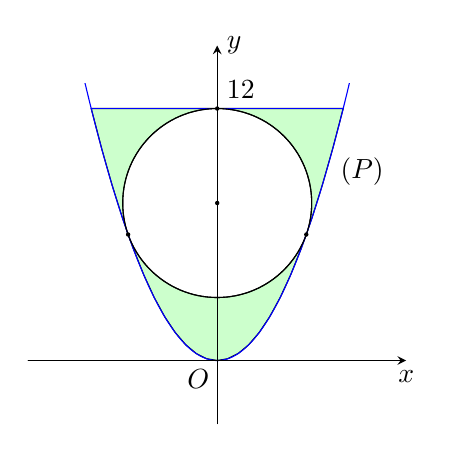
\begin{tikzpicture}[scale=.8, font=, line join=round, line cap=round, >=stealth]
			\pgfmathsetmacro\a{sqrt(2)}
			\begin{scope}
				\clip (-2.2,-0.7) rectangle (2.2,4.4);	
				\draw[fill=green!20] (2,4) -- (-2,4) -- plot[domain=-2:2] (\x, {(\x)^2}) -- cycle;	
				\draw[fill=white] (0,2.5) circle (1.5);		
				\draw[blue, domain=-2.2:2.2, samples=100] plot (\x, {(\x)^2});
			\end{scope}
			\draw[blue] (-2,4) -- (2,4);
			\draw (0,2.5) circle (1.5);
			\draw[->] (-3,0) -- (3,0) node[below] {$x$};
			\draw[->] (0,-1) -- (0,5) node[right] {$y$};
			\node at (-0.3,-0.3) {$O$};
			\node at (2.3, 3) {$(P)$};
			\fill[black] (0,4)node[above right]{$12$} circle (1pt)(0,2.5) circle (1pt) (-\a,2)circle (1pt) (\a,2)circle (1pt);
	\end{tikzpicture}}
	\par\shortans{24}
	\loigiai{
		Gọi $R$ là bán kính đường tròn $(C)$. Vì $(C)$ tiếp xúc với đường thẳng $y=12$ nên tọa độ tâm đường tròn $(C)$ là $I(0;12-R)$.\\
		Phương trình $(C)\colon x^2 + (y-12+R)^2 = R^2$.\\
		Thay $x^2 = \dfrac{y}{2}$ vào phương trình $(C)$, ta được
		$$\dfrac{y}{2}+y^2+144+R^2-24y+2Ry-24R = R^2 \Leftrightarrow 2y^2 + (4R-47)y + 288-48R = 0.$$
		Để $(C)$ tiếp xúc với $(P)$ thì phương trình trên có nghiệm kép, khi đó
		$$\Delta = (4R-47)^2 - 8(288-48R) = 0 \Leftrightarrow 16R^2+8R-95 = 0 \Rightarrow R=\dfrac{-1+4\sqrt{6}}{4}.$$
		Diện tích phần tô màu bằng diện tích hình phẳng giới hạn bởi $(P)$ và đường thẳng $y=12$ trừ đi diện tích hình tròn $(C)$.\\
		Phương trình hoành độ giao điểm của $(P)$ và đường thẳng $y=12$ là
		$$2x^2=12\Leftrightarrow x^2=6\Leftrightarrow x=\pm \sqrt{6}.$$
		Diện tích phần tô màu là
		$$S = \dfrac{2}{3}\cdot 2\sqrt{6}\cdot 12-\pi \left(\dfrac{-1+4\sqrt{6}}{4}\right)^2\approx 23{,}99\approx 24\, \left(\mathrm{cm}^2\right).$$
	}
\end{ex}

\begin{ex}%[0D0V2-4]%[TDMZZ28]%[Nguyễn Đức Tuấn Anh]
	Có $12$ người trong đó có $7$ nam và $5$ nữ bước ngẫu nhiên lên $4$ toa tàu khác nhau. Gọi $p$ là xác suất để mỗi toa tàu đều có $3$ người và đồng thời có cả nam và nữ. Hãy tính $10\,000p$ (\textit{không làm tròn ở các phép tính trung gian và làm tròn kết quả cuối cùng đến hàng đơn vị})?
	\begin{center}
		\begin{tikzpicture}[scale=1, line join=round, line cap=round, >=stealth, font=\footnotesize]
			\def\wheel#1#2{
				\filldraw[fill=black!80, draw=black, thick] (#1,#2) circle (0.28);
				\filldraw[fill=gray!40, draw=black, thin] (#1,#2) circle (0.18);
				\fill[black] (#1,#2) circle (0.06);
				\foreach \a in {0,45,...,315} {
					\draw[thin, gray!30] (#1,#2) -- ++(\a:0.18);
				}
			}
			\def\man#1#2{
				\fill[blue!70!black] (#1,#2+0.25) circle (0.12);
				\fill[blue!70!black, rounded corners=1pt] (#1-0.18,#2-0.2) rectangle (#1+0.18,#2+0.1);
			}
			\def\woman#1#2{
				\fill[red!70!black] (#1,#2+0.25) circle (0.12);
				\fill[red!70!black, rounded corners=1pt] (#1,#2+0.1) -- (#1-0.22,#2-0.2) -- (#1+0.22,#2-0.2) -- cycle;
			}
			
			\foreach \x in {-1,-0.5,...,16} {
				\fill[brown!80!black, rounded corners=1pt] (\x, -0.35) rectangle (\x+0.3, -0.2);
			}
			\draw[thick, double=gray!50, double distance=2pt] (-1, -0.18) -- (16.5, -0.18);
			\def\M{M}
			\foreach \i/\gA/\gB/\gC in {1/1/0/1, 2/1/1/0, 3/0/1/0, 4/0/1/1} {
				\pgfmathsetmacro{\x}{3*(\i-1)}
				\ifnum\i>1 
				\draw[line width=3pt, gray!60] (\x-0.4, 0.4) -- (\x, 0.4); 
				\fi
				\filldraw[fill=blue!10!white, draw=blue!40!black, thick, rounded corners=2pt] (\x, 0.35) rectangle (\x+2.6, 1.9);
				\filldraw[fill=red!60!black, draw=black, thick] (\x-0.1, 1.9) rectangle (\x+2.7, 2.15);
				\wheel{\x+0.5}{0.1}
				\wheel{\x+2.1}{0.1}
				\node[font=\bfseries\small, text=blue!80!black] at (\x+1.3, 0.55) {Toa \i};
				\foreach \w/\g in {1/\gA, 2/\gB, 3/\gC} {
					\pgfmathsetmacro{\wx}{\x + 0.3 + 0.75*(\w-1)}
					\filldraw[fill=cyan!5!white, draw=gray] (\wx, 0.8) rectangle (\wx+0.5, 1.5);
					\ifnum\g=1
					\man{\wx+0.25}{1.0}
					\else
					\woman{\wx+0.25}{1.0}
					\fi
				}
			}
			\draw[line width=3pt, gray!60] (11.6, 0.4) -- (12, 0.4);
			\filldraw[fill=black!80, draw=black, thick, rounded corners=2pt] (12, 0.35) rectangle (15.0, 1.5);
			\filldraw[fill=red!70!black, draw=black, thick] (12.0, 1.5) rectangle (13.2, 2.5);
			\filldraw[fill=black!90, draw=black] (11.8, 2.5) rectangle (13.4, 2.7);
			\filldraw[fill=cyan!10, draw=black, thick] (12.3, 1.7) rectangle (12.9, 2.3);
			\filldraw[fill=red!70!black, draw=black, thick] (14.2, 1.5) rectangle (14.6, 2.3);
			\filldraw[fill=orange!80!yellow, draw=black, thick] (14.1, 2.3) rectangle (14.7, 2.5);
			\filldraw[fill=orange!80!yellow, draw=black, thick] (13.4, 1.5) arc (180:0:0.25);
			\wheel{12.6}{0.1}
			\wheel{13.6}{0.1}
			\wheel{14.6}{0.1}
			\fill[gray!60, opacity=0.8] (14.4, 2.8) circle (0.25);
			\fill[gray!50, opacity=0.7] (14.1, 3.3) circle (0.35);
			\fill[gray!40, opacity=0.6] (13.6, 3.9) circle (0.45);
			\fill[gray!30, opacity=0.5] (12.9, 4.6) circle (0.6);
			\begin{scope}[shift={(6, 3.5)}]
				\draw[thick, rounded corners=2pt,  fill=white] (-1, -0.5) rectangle (2.6, 0.6);
				\man{-0.5}{0} \node[right] at (-.4, 0) {: Nam};
				\woman{1.4}{0} \node[right] at (1.5, 0) {: Nữ};
			\end{scope}
		\end{tikzpicture}
	\end{center}
	\par\shortans{90}
	\loigiai{
		Mỗi người có $4$ cách chọn toa tàu để bước lên. \\
		Do đó, số phần tử của không gian mẫu là $n(\Omega) = 4^{12} = 16\,777\,216$.\\
		Gọi $A$ là biến cố \lq\lq Mỗi toa tàu đều có $3$ người và đồng thời có cả nam và nữ\rq\rq.\\
		Vì mỗi toa có đúng $3$ người và có cả nam lẫn nữ nên số lượng nam, nữ trong một toa chỉ có thể là ($2$ nam, $1$ nữ) hoặc ($1$ nam, $2$ nữ).\\
		Gọi $x$ là số toa có $2$ nam, $1$ nữ và $y$ là số toa có $1$ nam, $2$ nữ ($x, y \in \mathbb{N}$). \\
		Ta có hệ phương trình
		\[\heva{&x + y = 4 \\&2x + y = 7} \Leftrightarrow \heva{&x = 3\\&y = 1.}\]
		Như vậy, có đúng $3$ toa xếp ($2$ nam, $1$ nữ) và $1$ toa xếp ($1$ nam, $2$ nữ).\\
		Khi đó, ta xếp người thỏa mãn biến cố $A$ như sau
		\begin{itemize}
			\item \textbf{Bước 1:} Chọn $1$ toa (trong $4$ toa) để xếp $1$ nam và $2$ nữ, có $\mathrm{C}_4^1 = 4$ cách ($3$ toa còn lại tự động được xếp $2$ nam và $1$ nữ).
			\item \textbf{Bước 2:} Phân bố $7$ nam vào $4$ toa. \\
			Chọn $1$ nam cho toa đặc biệt (ở Bước 1) có $\mathrm{C}_7^1$ cách.\\
			Chọn lần lượt $2$ nam cho $3$ toa còn lại có $\mathrm{C}_6^2 \cdot \mathrm{C}_4^2 \cdot \mathrm{C}_2^2$ cách. \\
			Số cách xếp nam là $7 \cdot 15 \cdot 6 \cdot 1 = 630$ cách.
			\item \textbf{Bước 3:} Phân bố $5$ nữ vào $4$ toa. \\
			Chọn $2$ nữ cho toa đặc biệt có $\mathrm{C}_5^2$ cách. \\
			Chọn lần lượt $1$ nữ cho $3$ toa còn lại có $\mathrm{C}_3^1 \cdot \mathrm{C}_2^1 \cdot \mathrm{C}_1^1$ cách. \\
			Số cách xếp nữ là $10 \cdot 3 \cdot 2 \cdot 1 = 60$ cách.
		\end{itemize}
		Số kết quả thuận lợi cho biến cố $A$ là $n(A) = 4 \cdot 630 \cdot 60 = 151\,200$.\\
		Xác suất của biến cố $A$ là $p = \dfrac{n(A)}{n(\Omega)} = \dfrac{151\,200}{16\,777\,216}$.\\
		Suy ra $10\,000p = 10\,000 \cdot \dfrac{151\,200}{16\,777\,216} \approx 90$.
	}
\end{ex}
\begin{ex}
	content
\end{ex}
\begin{ex}%[0D0C2-5]%[TDM42]%[Nguyễn Văn Sang]
	Để chuẩn bị giao nhiệm vụ cho hai bạn thực tập viên An và Bình, người ta đã chuẩn bị sẵn $36$ phong bì thư giống nhau, bên trong có $10$ công việc khó (coi như giống nhau) và $26$ công việc bình thường (coi như giống nhau). Bạn An chọn ngẫu nhiên $10$ phong bì (có hoàn lại), sau đó bạn Bình chọn ngẫu nhiên $6$ phong bì.\\
	Gọi $p$ là xác suất để bạn An được giao $4$ công việc khó và bạn Bình được giao $1$ công việc khó, nếu đã biết sau khi hai bạn chọn ngẫu nhiên các phong bì thì còn $23$ phong bì chưa được bạn nào chọn. Hãy tính $1000p$ (làm tròn kết quả đến hàng đơn vị)?
	\begin{center}
		\begin{tikzpicture}[scale=0.7, >=stealth]
			% Phong bì đỏ (Công việc khó)
			\draw[fill=yellow!20, draw=orange, thick] (1, 7.5) -- (2.5, 8.8) -- (4, 7.5) -- cycle;
			\draw[fill=red!80, draw=red, thick, rounded corners=2pt] (1.2, 6.5) rectangle (3.8, 8.5);
			% \node[white, align=center, scale=0.85] at (2.5, 7.8) {\textbf{CÔNG VIỆC}\\\textbf{KHÓ}};
			\draw[fill=yellow!30, draw=orange, thick, rounded corners=2pt] (1, 6) rectangle (4, 7.5);
			\draw[orange, thick] (1, 7.5) -- (2.5, 6.5) -- (4, 7.5);
			\draw[orange, thick] (1, 6) -- (2.5, 6.5) -- (4, 6);
			
			\node[red, align=center] at (-1.5, 7.5) {\textbf{10 công việc}\\\textbf{khó (màu đỏ)}};
			% \node[red, scale=1.5] at (-0.5, 6.5) {\textbf{10}};
			\draw[->, red, thick] (0.5, 7.5) to[out=20, in=160] (1.2, 7.5);
			
			% Phong bì xanh (Công việc bình thường)
			\draw[fill=yellow!20, draw=orange, thick] (5, 7.5) -- (6.5, 8.8) -- (8, 7.5) -- cycle;
			\draw[fill=blue!70, draw=blue, thick, rounded corners=2pt] (5.2, 6.5) rectangle (7.8, 8.5);
			% \node[white, align=center, scale=0.75] at (6.5, 7.8) {\textbf{CÔNG VIỆC}\\\textbf{BÌNH THƯỜNG}};
			\draw[fill=yellow!30, draw=orange, thick, rounded corners=2pt] (5, 6) rectangle (8, 7.5);
			\draw[orange, thick] (5, 7.5) -- (6.5, 6.5) -- (8, 7.5);
			\draw[orange, thick] (5, 6) -- (6.5, 6.5) -- (8, 6);
			
			\node[blue, align=center] at (13, 7.5) {\textbf{26 công việc}\\\textbf{bình thường (màu xanh)}};
			% \node[blue, scale=1.5] at (9.5, 6.5) {\textbf{26}};
			\draw[<-, blue, thick] (7.8, 7.5) to[out=20, in=160] (8.5, 7.5);
			
			% Khung bao 36 phong bì
			\node at (4.5, 4.8) {\textbf{36 phong bì thư giống nhau}};
			\draw[thick, blue!50] (-0.5, 4.8) -- (1.5, 4.8);
			\draw[thick, blue!50] (7.5, 4.8) -- (9.5, 4.8);
			
			\draw[thick, blue!50, rounded corners=5pt] (-0.5, 1) rectangle (9.5, 4.5);
			
			% Các phong bì nhỏ
			\foreach \r in {1,2,3,4} {
				\foreach \c in {1,...,9} {
					\pgfmathsetmacro{\x}{-0.2 + (\c-1)*1.1}
					\pgfmathsetmacro{\y}{4.2 - (\r-1)*0.8}
					\draw[fill=yellow!20, draw=orange, rounded corners=1pt] (\x, \y-0.5) rectangle ++(0.8, 0.5);
					\draw[orange] (\x, \y) -- ++(0.4, -0.25) -- ++(0.4, 0.25);
					\fill[red] (\x+0.4, \y-0.25) circle (0.04);
				}
			}
		\end{tikzpicture}
	\end{center}
	\par\shortans[0]{56}
	\loigiai{
		\textbf{Cách tiếp cận:} Để bài toán đơn giản và dễ hiểu, ta có thể tưởng tượng quá trình diễn ra theo 2 giai đoạn:\\
		- \textbf{Giai đoạn 1:} An và Bình chọn các phong bì. Lúc này, ta chưa cần quan tâm bên trong phong bì có gì. Các phong bì được chia thành các nhóm tùy theo việc ai đã chọn nó.\\
		- \textbf{Giai đoạn 2:} Bỏ ngẫu nhiên $10$ công việc khó (CVK) và $26$ công việc bình thường (CVBT) vào 36 phong bì đó (mỗi phong bì 1 công việc). Ta sẽ tính xác suất để số CVK rơi vào các nhóm đúng theo yêu cầu.\\
		\textbf{Bước 1: Phân chia 36 phong bì thành các nhóm (Giai đoạn 1)}\\
		Hành động "chọn có hoàn lại" nghĩa là An chọn xong, ghi nhận lại rồi trả vào, sau đó Bình mới chọn. Do đó, mỗi phong bì sẽ rơi vào 1 trong 4 nhóm sau:
		\begin{itemize}
			\item Nhóm 1: Được cả An và Bình chọn.
			\item Nhóm 2: Chỉ được An chọn.
			\item Nhóm 3: Chỉ được Bình chọn.
			\item Nhóm 4: Không được ai chọn.
		\end{itemize}
		Theo giả thiết\\
		- Nhóm 4 có $23$ phong bì.\\
		- Tổng số phong bì được ít nhất một người chọn (gồm Nhóm 1, 2, 3) là $36 - 23 = 13$ phong bì.\\
		- Mặt khác, tổng số lượt chọn của An và Bình là $10 + 6 = 16$.\\
		Số lượt chọn dư ra so với số phong bì thực tế được chọn chính là số phong bì bị chọn trùng (Nhóm 1).\\
		Suy ra\\
		- Số phong bì Nhóm 1 (cả 2 cùng chọn): $16 - 13 = 3$ phong bì.\\
		- Số phong bì Nhóm 2 (chỉ An chọn): $10 - 3 = 7$ phong bì.\\
		- Số phong bì Nhóm 3 (chỉ Bình chọn): $6 - 3 = 3$ phong bì.\\
		\textbf{Bước 2: Phân bổ công việc vào các nhóm (Giai đoạn 2)}\\
		Việc xếp $10$ CVK vào $36$ phong bì chính là chọn ngẫu nhiên $10$ phong bì để chứa CVK. Các phong bì còn lại mặc nhiên chứa CVBT.\\
		Không gian mẫu lúc này (số cách chọn 10 phong bì từ 36 phong bì) là
		$$n(\Omega) = \mathrm{C}_{36}^{10} = 254\,186\,856.$$
		Ta cần phân bổ 10 CVK sao cho: An có 4 CVK, Bình có 1 CVK.\\
		Gọi $x$ là số CVK rơi vào Nhóm 1. Vì Bình chỉ có 1 CVK nên $x \le 1 \Rightarrow x \in \{0; 1\}$.
		\begin{itemize}
			\item \textbf{Trường hợp 1: $x = 0$ (Nhóm 1 không có CVK nào)}\\
			- Nhóm 1 (3 pb): 0 CVK.\\
			- Nhóm 2 (7 pb): Để An có 4 CVK, nhóm này cần có $4 - 0 = 4$ CVK.\\
			- Nhóm 3 (3 pb): Để Bình có 1 CVK, nhóm này cần có $1 - 0 = 1$ CVK.\\
			- Nhóm 4 (23 pb): Nhận số CVK còn lại là $10 - (0+4+1) = 5$ CVK.\\
			Số cách chọn phong bì chứa CVK cho trường hợp này là:
			$$W_1 = \mathrm{C}_3^0 \cdot \mathrm{C}_7^4 \cdot \mathrm{C}_3^1 \cdot \mathrm{C}_{23}^5 = 1 \cdot 35 \cdot 3 \cdot 33\,649 = 3\,533\,145 \text{ (cách)}$$
			\item \textbf{Trường hợp 2: $x = 1$ (Nhóm 1 có 1 CVK)}\\
			- Nhóm 1 (3 pb): 1 CVK.\\
			- Nhóm 2 (7 pb): An cần thêm $4 - 1 = 3$ CVK.\\
			- Nhóm 3 (3 pb): Bình cần thêm $1 - 1 = 0$ CVK.\\
			- Nhóm 4 (23 pb): Nhận số CVK còn lại là $10 - (1+3+0) = 6$ CVK.\\
			Số cách chọn phong bì chứa CVK cho trường hợp này là:
			$$W_2 = \mathrm{C}_3^1 \cdot \mathrm{C}_7^3 \cdot \mathrm{C}_3^0 \cdot \mathrm{C}_{23}^6 = 3 \cdot 35 \cdot 1 \cdot 100\,947 = 10\,599\,435 \text{ (cách)}$$
		\end{itemize}
		Tổng số cách phân bổ thỏa mãn là
		$$n(A) = W_1 + W_2 = 3\,533\,145 + 10\,599\,435 = 14\,132\,580 \text{ (cách)}$$
		\textbf{Bước 3: Tính xác suất}\\
		Xác suất để xảy ra yêu cầu của bài toán là
		$$p = \dfrac{n(A)}{n(\Omega)} = \dfrac{14\,132\,580}{254\,186\,856} = \dfrac{15295}{275094} \approx 0,055599$$
		Vậy $1000p \approx 55,599$. Làm tròn kết quả đến hàng đơn vị, ta được $\boxed{56}$.
	}
\end{ex}